\chapter{Конструкторский раздел}
\section{Разработка алгоритмов}
В разделе представлены схемы следующих алгоритмов вычисления расстояния:
\begin{itemize}
	\item Левенштейна обычным способом (матричным) (рисунки 2.1-2.2)
	\item Левенштейна рекурсивным способом (рисунки 2.3-2.4)
	\item Левенштейна рекурсивным способом с кэшированием (рисунки 2.5-2.6)
	\item Дамерау-Левенштейна обычным способом (матричным) (рисунки 2.7-2.8)
\end{itemize}

\begin{figure}
	\center{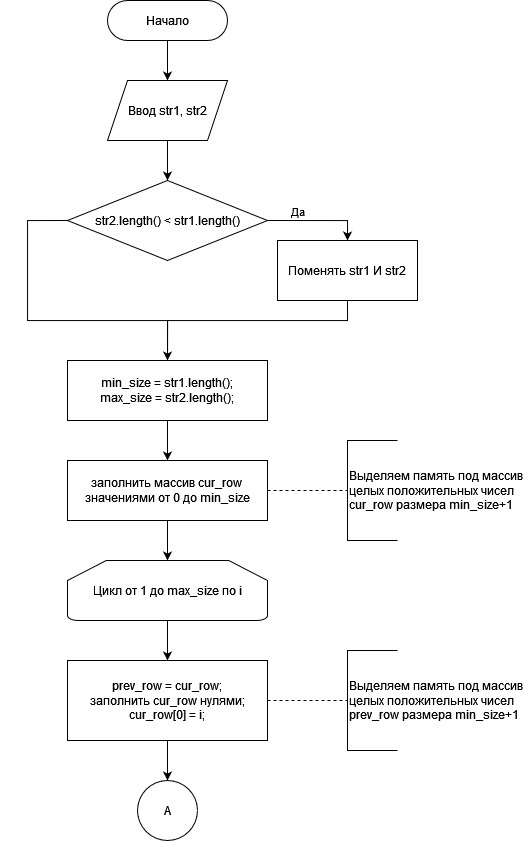
\includegraphics[width=0.93\linewidth]{inc/img/LevLen1}}
	\caption{Схема алгоритма Левенштейна часть 1}
\end{figure}

\begin{figure}
	\center{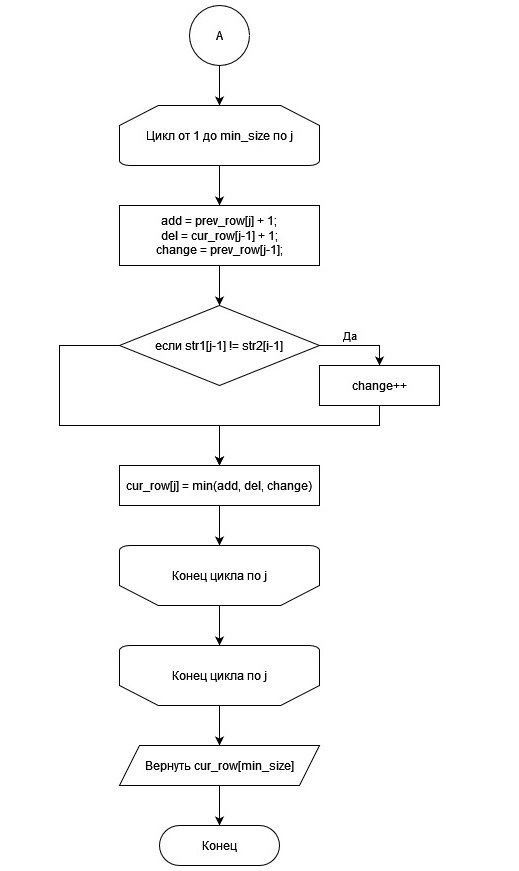
\includegraphics[width=0.93\linewidth]{inc/img/LevLen2}}
	\caption{Схема алгоритма Левенштейна часть 2}
\end{figure}

\begin{figure}
	\center{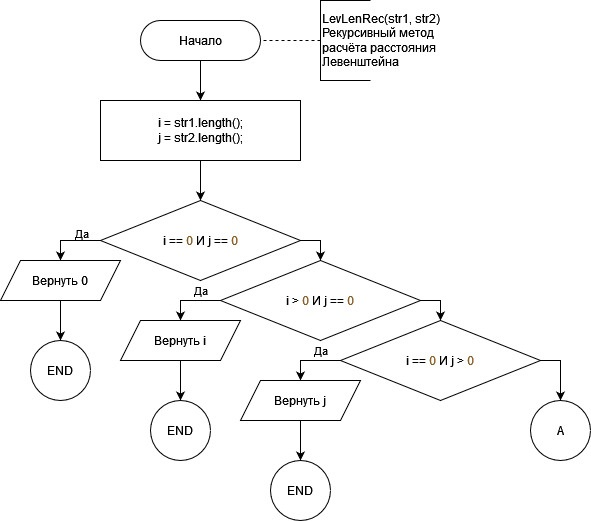
\includegraphics[width=0.93\linewidth]{inc/img/LevLenRec1}}
	\caption{Схема алгоритма Левенштейна с рекурсией часть 1}
\end{figure}

\begin{figure}
	\center{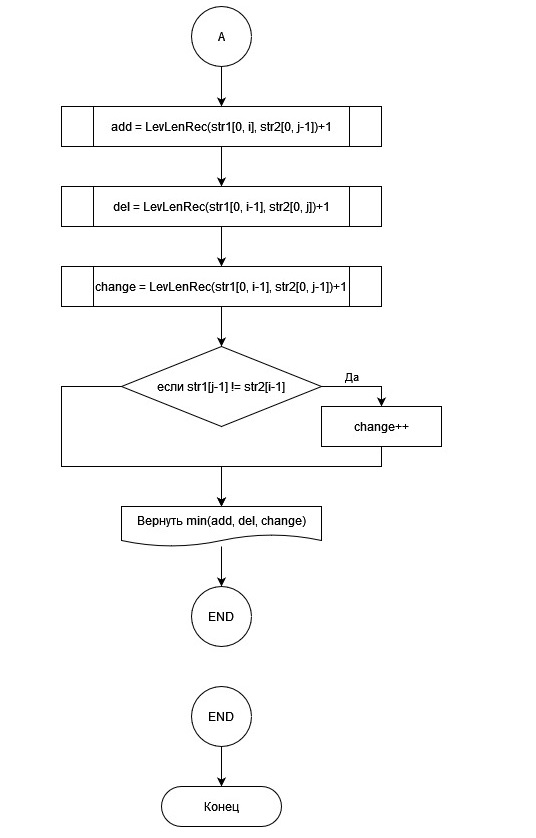
\includegraphics[width=0.93\linewidth]{inc/img/LevLenRec2}}
	\caption{Схема алгоритма Левенштейна с рекурсией часть 2}
\end{figure}

\begin{figure}
	\center{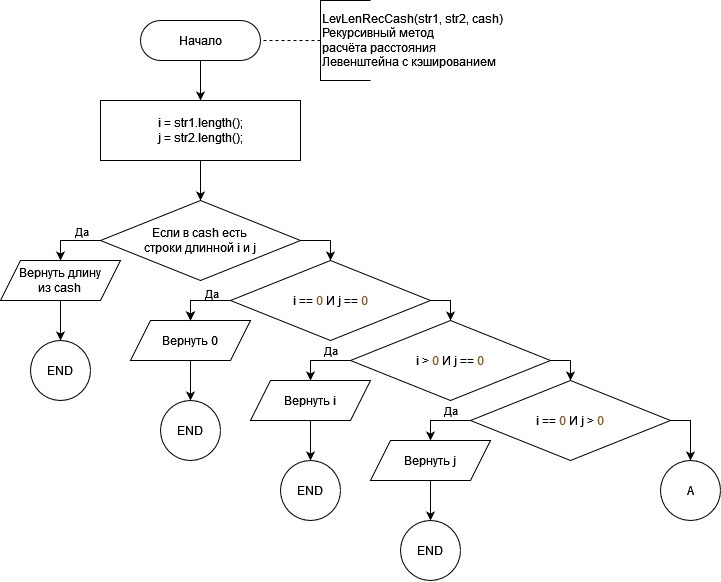
\includegraphics[width=0.93\linewidth]{inc/img/LevLenRecCash1}}
	\caption{Схема алгоритма Левенштейна с рекурсией и кэшированием часть 1}
\end{figure}

\begin{figure}
	\center{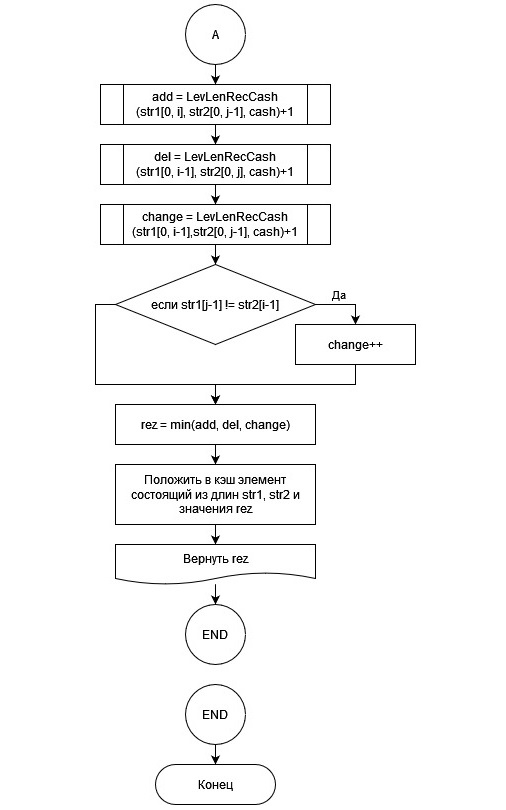
\includegraphics[width=0.93\linewidth]{inc/img/LevLenRecCash2}}
	\caption{Схема алгоритма Левенштейна с рекурсией и кэшированием часть 2}
\end{figure}

\begin{figure}
	\center{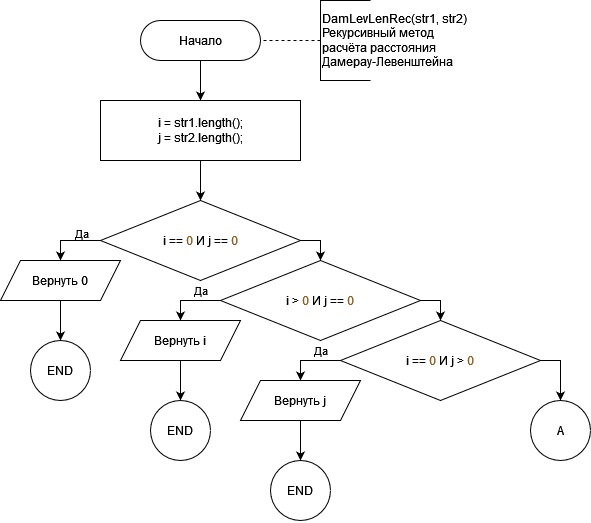
\includegraphics[width=0.93\linewidth]{inc/img/DamLevLenRec1}}
	\caption{Схема алгоритма Дамерау-Левенштейна с рекурсией часть 1}
\end{figure}

\begin{figure}
	\center{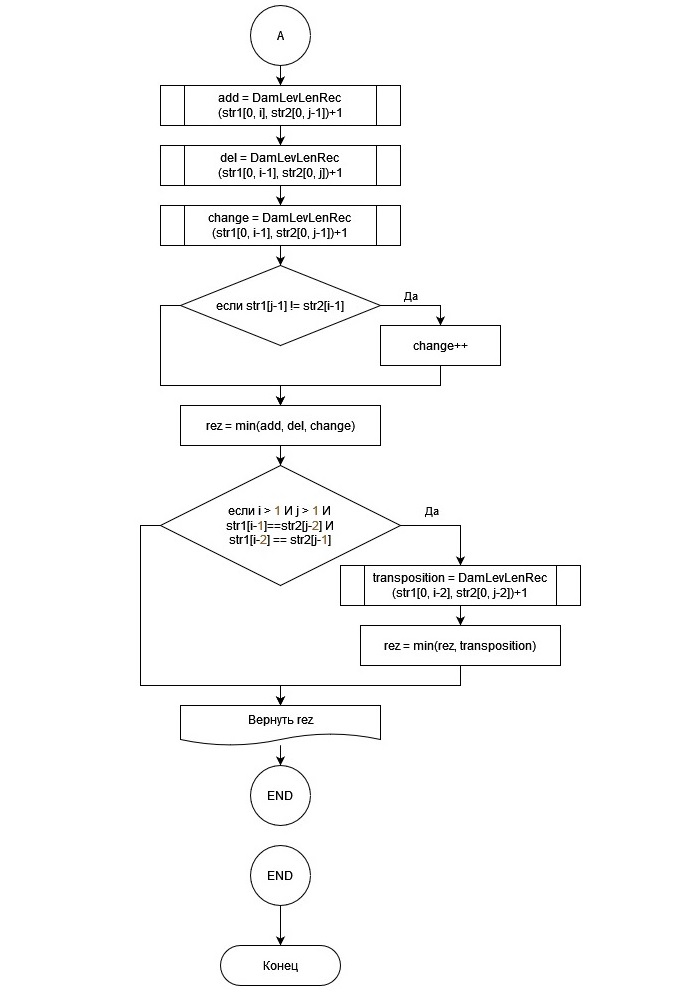
\includegraphics[width=0.93\linewidth]{inc/img/DamLevLenRec2}}
	\caption{Схема алгоритма Дамерау-Левенштейна с рекурсией часть 2}
\end{figure}

\newpage